\documentclass[a4paper,12pt]{article}
\usepackage{graphicx}
\usepackage{apacite}
\bibliographystyle{apacite}
\usepackage{titlepic}

\begin{document}

% Configuración de la portada
\begin{titlepage}
    \centering
    \vspace*{2cm}

    % Título
    {\Huge \textbf{Movimiento Semiparabólico}} \\[1.5cm]

    % Subtítulo (opcional)
    {\Large \textbf{Análisis y Aplicaciones}} \\[1.5cm]

    % Autor
    {\large Autor: Marco Beltrán y Stiven Mmmm} \\[0.5cm]

    % Fecha
    {\large Fecha: 17 de septiembre de 2024} \\[2cm]

    % Imagen (opcional)
    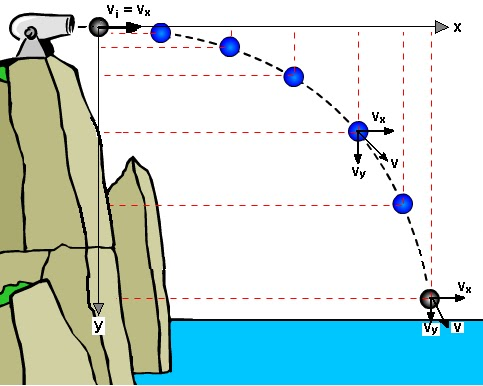
\includegraphics[width=0.4\textwidth]{imagenes/Dibujo1.jpg} \\[1cm]

    % Institución
    {\large \textbf{Universidad Distrital Francisco José de Caldas}} \\[0.5cm]

    % Footer
    \vfill
    {\large Página 1}
\end{titlepage}

% No es necesario repetir \begin{document}
% Título y autor (opcional)
\title{Informe de Laboratorio: Movimiento Semiparabólico}
\author{}
\date{}
\maketitle

\section{Marco Teórico}
El movimiento semiparabólico describe el movimiento de un cuerpo que sigue una trayectoria curva bajo la influencia de un campo gravitacional uniforme, con desplazamiento limitado o controlado en la dirección vertical. Este tipo de movimiento se puede analizar descomponiendo el desplazamiento en dos componentes: horizontal y vertical.

En la dirección horizontal, al no haber aceleración (si se desprecia la resistencia del aire), el movimiento es rectilíneo uniforme, lo que se expresa mediante:

\[
x(t) = v_{0x} \cdot t
\]

Donde:
\begin{itemize}
    \item $x(t)$ es la posición horizontal en el tiempo $t$.
    \item $v_{0x}$ es la velocidad inicial en la dirección horizontal.
\end{itemize}

En la dirección vertical, el movimiento está influenciado por la aceleración debido a la gravedad $g$, que produce un movimiento uniformemente acelerado. La ecuación para la posición vertical $y(t)$ es:

\[
y(t) = y_0 + v_{0y} \cdot t - \frac{1}{2} g t^2
\]

Donde:
\begin{itemize}
    \item $y(t)$ es la posición vertical en el tiempo $t$.
    \item $y_0$ es la altura inicial.
    \item $v_{0y}$ es la velocidad inicial en la dirección vertical (que en muchos casos puede ser cero).
    \item $g$ es la aceleración debida a la gravedad (aproximadamente $9.81 \, \text{m/s}^2$).
\end{itemize}

La trayectoria del movimiento resulta ser una parábola parcial cuando las dos componentes se combinan.

\section{Relevancia del Experimento}
La realización de este experimento es fundamental para comprender cómo interactúan las componentes de un movimiento en dos dimensiones, específicamente cómo se combinan el movimiento rectilíneo uniforme (en la dirección horizontal) y el movimiento uniformemente acelerado (en la dirección vertical) para formar una trayectoria semiparabólica. Estudiar este tipo de movimiento permite una mejor comprensión de la dinámica de objetos en campos gravitacionales y es aplicable en áreas como la ingeniería balística, deportes y cualquier fenómeno relacionado con trayectorias de cuerpos en el aire. Además, su análisis permite profundizar en conceptos clave como la independencia de los movimientos y las ecuaciones de cinemática.

\section{Propósito}
El objetivo de este experimento es investigar las características del movimiento semiparabólico y comprobar la relación entre los tiempos de caída, la altura y la velocidad horizontal del objeto. Se espera comprobar que el movimiento en la dirección horizontal es independiente del movimiento vertical y que la aceleración debido a la gravedad solo afecta al desplazamiento vertical.

Para calcular el tiempo de vuelo $t_{\text{vuelo}}$, se utiliza la ecuación para la posición vertical igualando $y(t)$ a 0 (asumiendo que el objeto cae al suelo desde una altura $y_0$):

\[
t_{\text{vuelo}} = \sqrt{\frac{2 y_0}{g}}
\]

Con este tiempo, es posible determinar el alcance horizontal máximo $x_{\text{max}}$:

\[
x_{\text{max}} = v_{0x} \cdot t_{\text{vuelo}}
\]

A través de mediciones experimentales, se pretende validar estas ecuaciones teóricas que describen el movimiento y obtener conclusiones sobre los factores que influyen en la trayectoria.

\section*{Objetivos}

El presente trabajo tiene como objetivo realizar un análisis detallado del movimiento semiparabólico de dos esferas de diferentes tamaños. A partir de este análisis, se busca obtener y calcular los siguientes datos:

\begin{itemize}
    \item \textbf{Masa de cada esfera:} Determinar y registrar la masa de cada esfera utilizada en el experimento, lo cual es fundamental para entender la dinámica del movimiento.
    
    \item \textbf{Radio de cada esfera:} Medir y documentar el radio de ambas esferas, ya que este parámetro influye en la forma en que cada esfera se comporta al ser lanzada.

    \item \textbf{Alcance:} Calcular el alcance horizontal de cada esfera, que representa la distancia máxima recorrida en la dirección horizontal durante su trayectoria.

    \item \textbf{Altura máxima:} Establecer la altura máxima alcanzada por cada esfera en su trayectoria, lo cual proporciona información sobre la energía potencial en el sistema.

    \item \textbf{Tiempo de vuelo:} Medir el tiempo total de vuelo de cada esfera, permitiendo analizar la relación entre el tiempo y los otros parámetros del movimiento.
\end{itemize}

\section{Materiales}

A continuación se detallan los materiales utilizados en el experimento, incluyendo imágenes de cada uno y su respectiva adaptación:

\begin{itemize}
    \item \textbf{Material} \\
    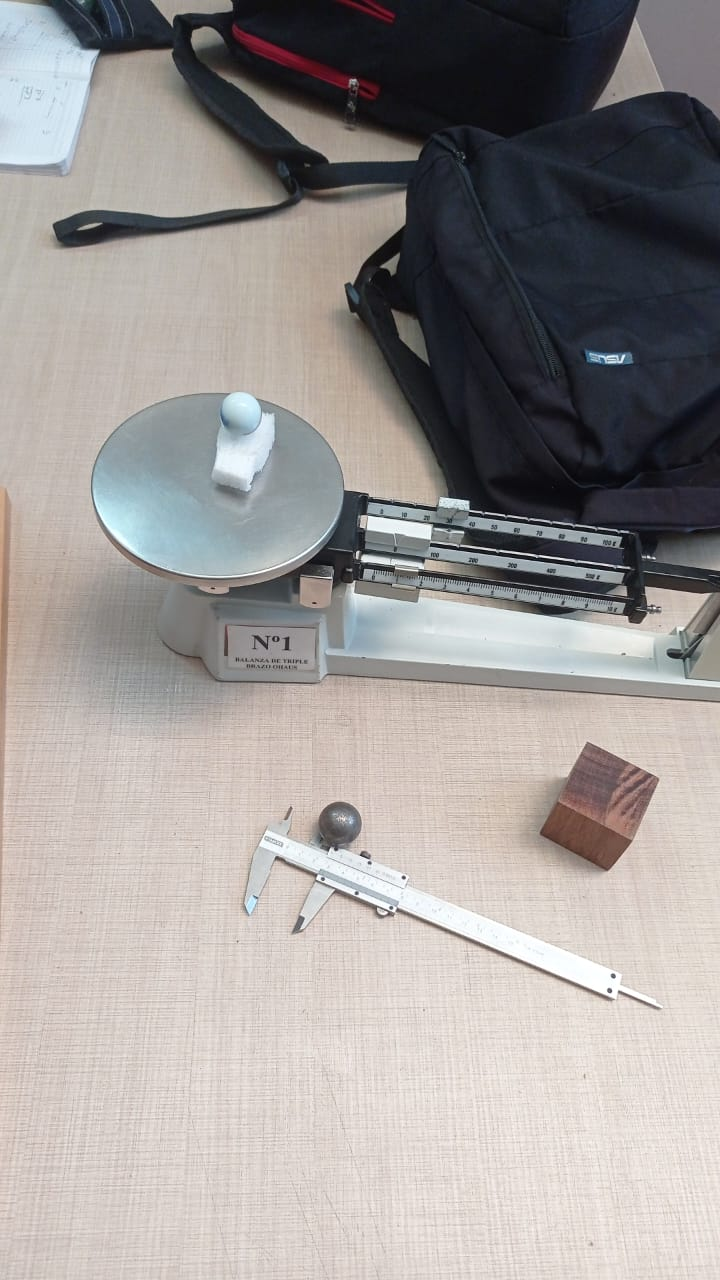
\includegraphics[width=0.9\textwidth]{imagenes/1.jpeg} \\
    Adaptación: PESA, CALIBRE, BASE Y ESFERAS.
    
    \vspace{0.5cm} % Espacio entre materiales

    \item \textbf{BASES:} \\
    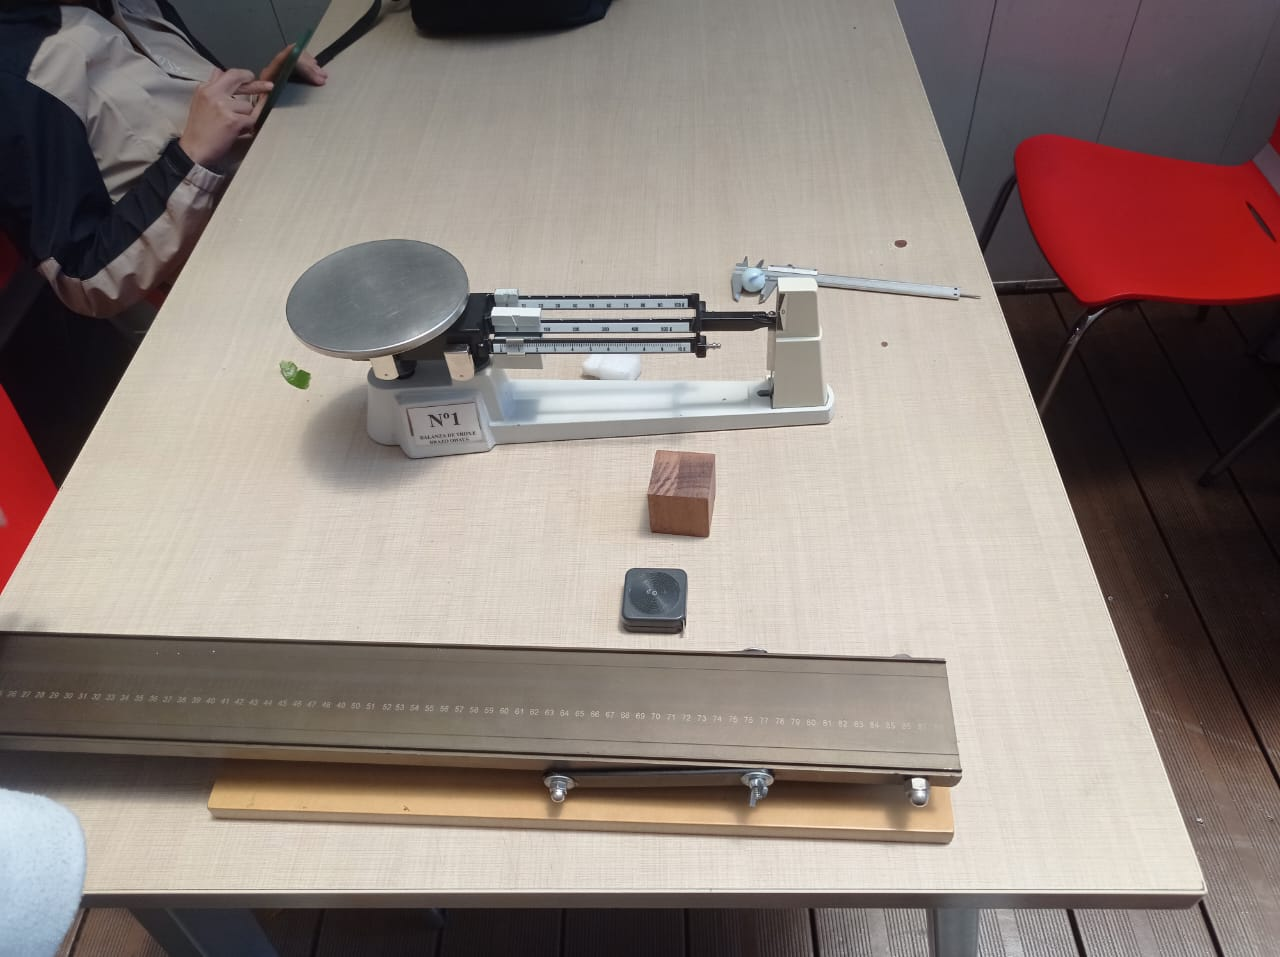
\includegraphics[width=0.9\textwidth]{imagenes/2.jpeg} \\
    Adaptación: Un sistema de referencia en física.

    \vspace{0.5cm}

    \item \textbf{MEDICION:} \\
    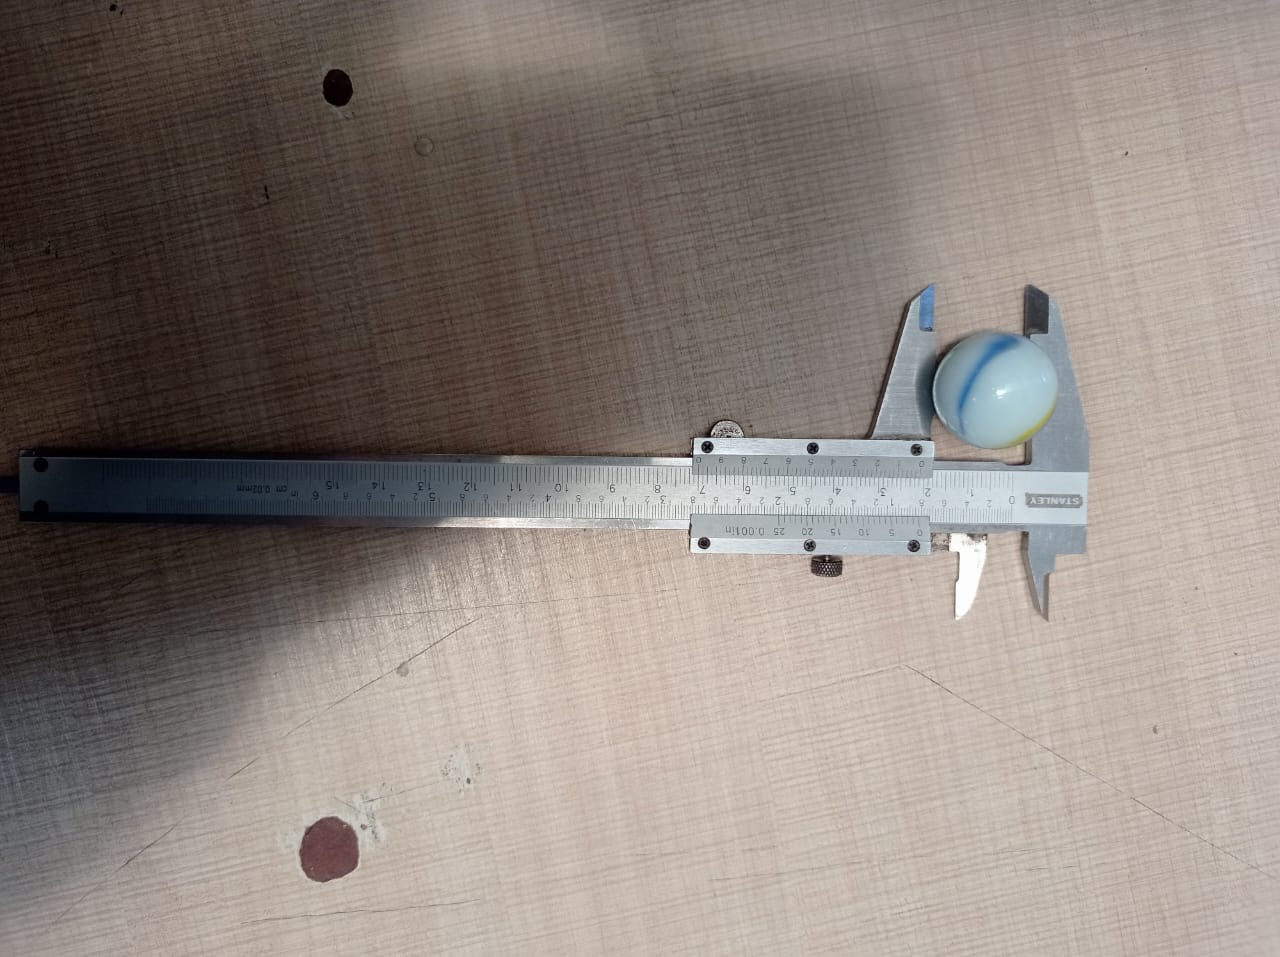
\includegraphics[width=0.9\textwidth]{imagenes/3.jpeg} \\
    Adaptación: herramienta utilizada en ingeniería y manufactura para medir dimensiones lineales

    \vspace{0.5cm}

    \item \textbf{MEDICON:} \\
    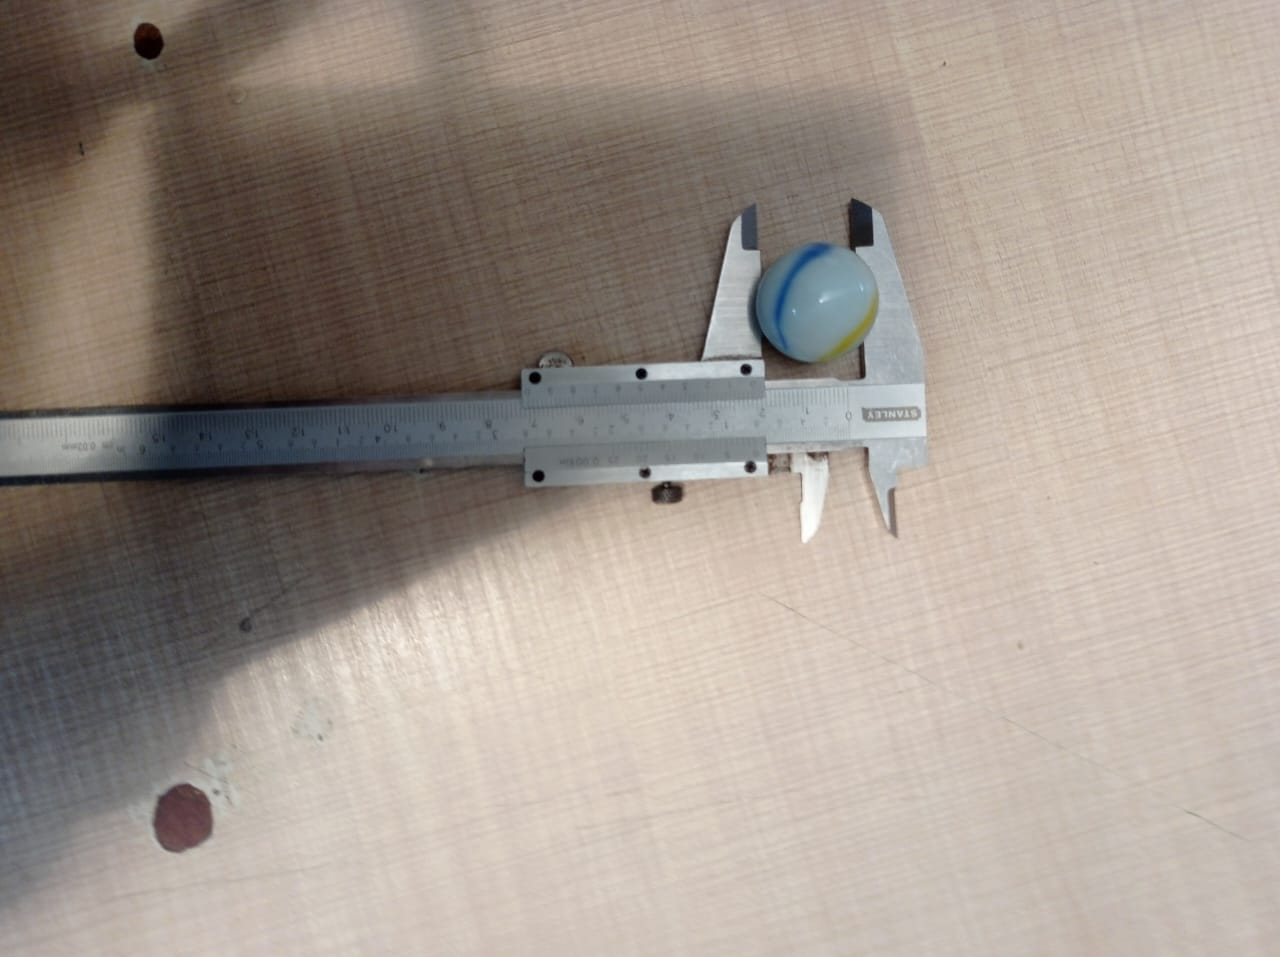
\includegraphics[width=0.9\textwidth]{imagenes/4.jpeg} \\
    Adaptación: herramienta utilizada en ingeniería y manufactura para medir dimensiones lineales.

    \vspace{0.5cm}

    \item \textbf{MEDICION:} \\
    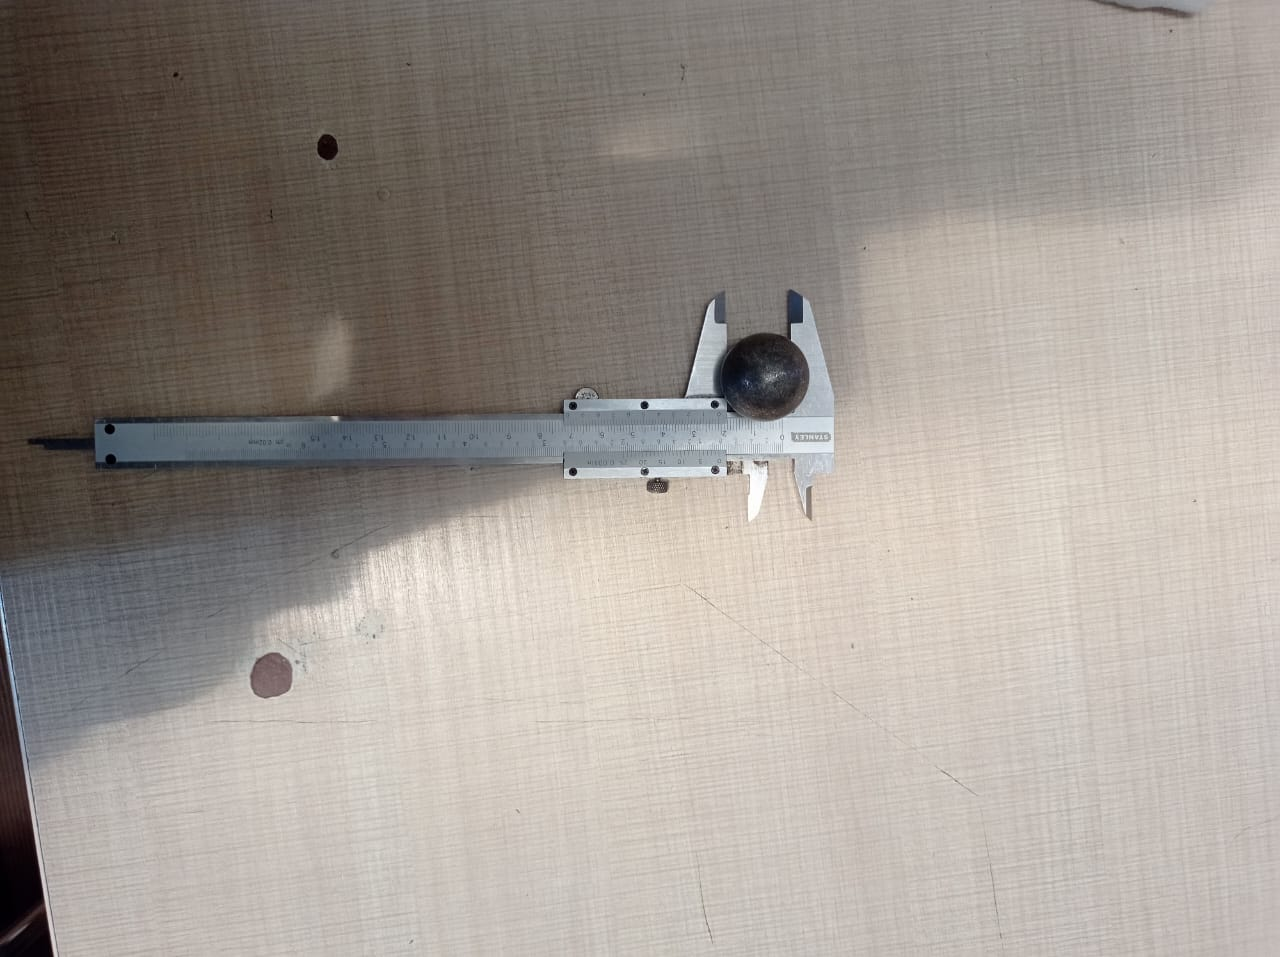
\includegraphics[width=0.9\textwidth]{imagenes/5.jpeg} \\
    Adaptación: herramienta utilizada para medir dimensiones lineales.

    \vspace{0.5cm}

    \item \textbf{MEDICON:} \\
    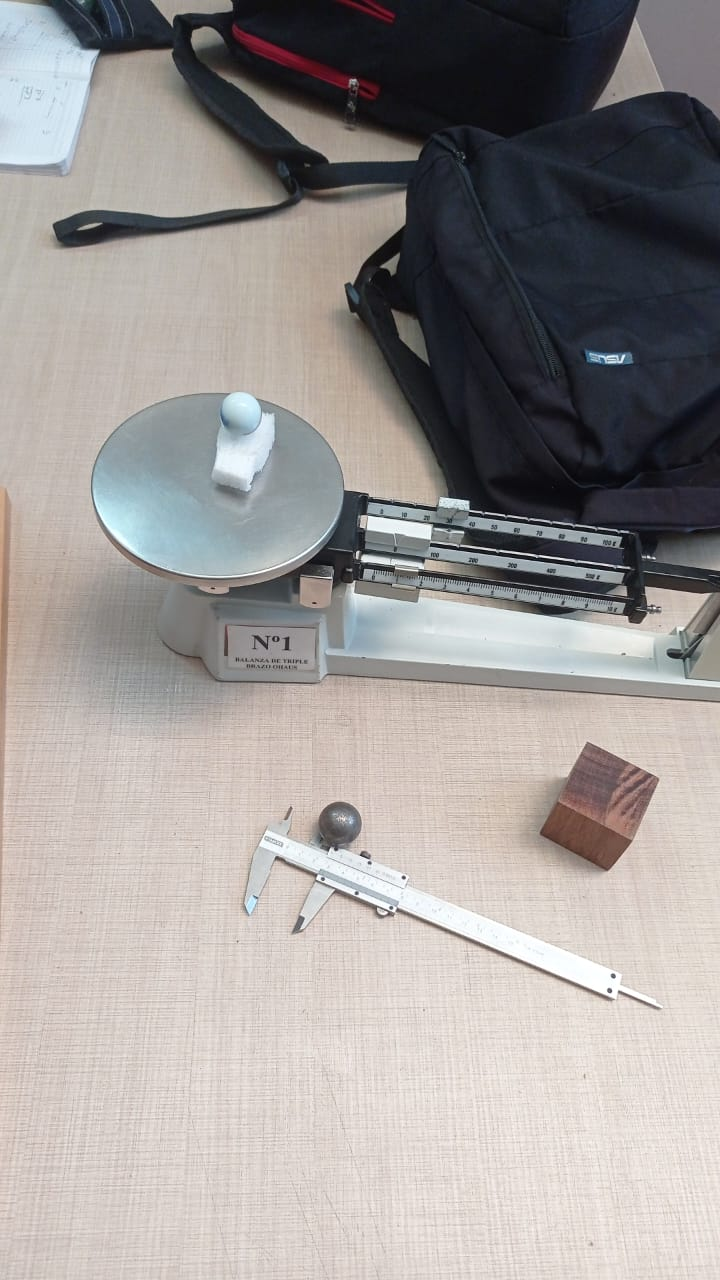
\includegraphics[width=0.9\textwidth]{imagenes/6.jpeg} \\
    Adaptación:Ofrece una alta precisión en la medición de masa .

    \vspace{0.5cm}

    \item \textbf{MEDICION:} \\
    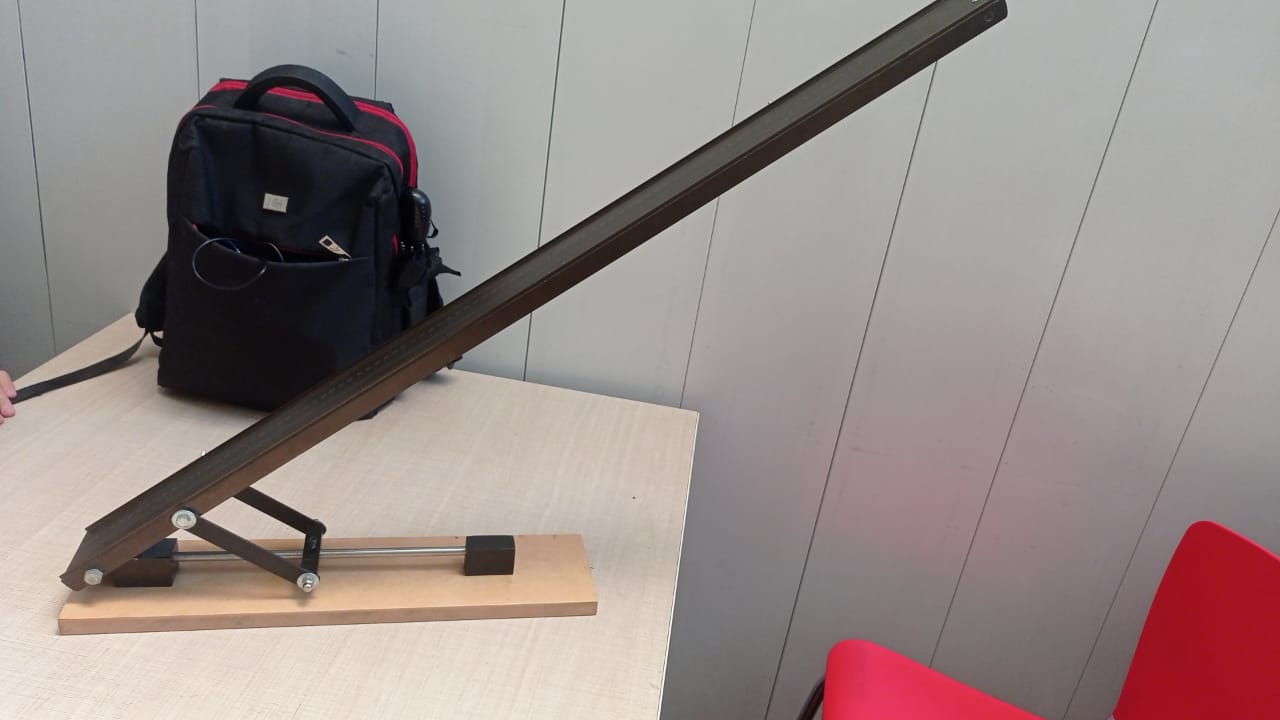
\includegraphics[width=0.9\textwidth]{imagenes/7.jpeg} \\
    Adaptación: BASE.
\end{itemize}

\section{Resultados}

A continuación se presentan los resultados obtenidos durante el experimento, incluyendo las mediciones de las esferas y el análisis del movimiento semiparabólico.

\subsection{Mediciones Generales}
\begin{itemize}
    \item Longitud del plano: 89 cm
    \item Altura del lanzamiento (H): 46.5 cm
    \item Despreciable: 5 cm
    \item Distancia en el plano: 15 cm
\end{itemize}

\subsection{Datos de las Esferas}
\begin{itemize}
    \item \textbf{Esfera 1:}
    \begin{itemize}
        \item Diámetro: 2.74 cm
        \item Tiempo de vuelo: 1.45 s
    \end{itemize}

    \item \textbf{Esfera 2:}
    \begin{itemize}
        \item Diámetro: 1.64 cm
        \item Masa: 20.07 g
        \item Tiempo de vuelo: 1.13 s
    \end{itemize}
\end{itemize}

\subsection{Cálculo del Ángulo}
Para determinar el ángulo de lanzamiento (\(\theta\)), se puede utilizar la siguiente relación:

\[
\tan(\theta) = \frac{H}{L}
\]

Donde:
- \(H\) es la altura de lanzamiento.
- \(L\) es la longitud del plano.

Sustituyendo los valores:

\[
\tan(\theta) = \frac{46.5 \, \text{cm}}{89 \, \text{cm}}
\]

Para encontrar el ángulo \(\theta\):

\[
\theta = \tan^{-1}\left(\frac{46.5}{89}\right) \approx 28.74^\circ
\]

Este cálculo muestra el ángulo de lanzamiento de las esferas durante el experimento.


% Título y autor (opcional)
\title{Informe de Laboratorio: Movimiento Semiparabólico}
\author{}
\date{}
\maketitle

\section{Datos del Experimento}

\subsection{Datos Generales}
\begin{table}[h!]
    \centering
    \begin{tabular}{l c}
        \toprule
        \textbf{Descripción} & \textbf{Valor} \\
        \midrule
        Longitud del plano & 89 cm \\
        Altura del lanzamiento (H) & 46.5 cm \\
        Despreciable & 5 cm \\
        Distancia en el plano & 15 cm \\
        \bottomrule
    \end{tabular}
    \caption{Datos generales del experimento}
    \label{tab:datos_generales}
\end{table}


\begin{table}[h!]
    \centering
    \begin{tabular}{l c c}
        \toprule
        \textbf{Esfera} & \textbf{Diámetro} & \textbf{Masa} & \textbf{Tiempo de Vuelo} \\
        \midrule
        Esfera 1 & 2.74 cm & -- & 1.45 s \\
        Esfera 2 & 1.64 cm & 20.07 g & 1.13 s \\
        \bottomrule
    \end{tabular}
    \caption{Datos de las esferas utilizadas en el experimento}
    \label{tab:datos_esferas}
\end{table}

\section{Conclusión}

El informe presenta un análisis exhaustivo del movimiento semiparabólico, un tipo de trayectoria curvada que sigue un objeto bajo la influencia de la gravedad. El movimiento se descompone en dos componentes: horizontal, que es rectilíneo uniforme, y vertical, que es uniformemente acelerado debido a la gravedad. Estas componentes se combinan para formar una trayectoria parabólica.

El experimento realizado permite validar las ecuaciones teóricas del movimiento semiparabólico, confirmando que el movimiento horizontal es independiente del vertical y que la aceleración gravitacional afecta únicamente el desplazamiento vertical. Se midieron y analizaron diversas características de las esferas utilizadas, como masa, diámetro, alcance, altura máxima y tiempo de vuelo.

Los resultados obtenidos coinciden con las predicciones teóricas. Se calculó el ángulo de lanzamiento, que fue de aproximadamente 28.74 grados, basándose en la altura de lanzamiento y la longitud del plano. Estos hallazgos son cruciales para comprender mejor la dinámica del movimiento en dos dimensiones y tienen aplicaciones prácticas en campos como la ingeniería balística y el análisis de trayectorias en deportes.

El experimento demuestra cómo el análisis teórico del movimiento semiparabólico se puede aplicar y verificar mediante la experimentación práctica, destacando la importancia de entender la interacción entre las componentes horizontal y vertical del movimiento.


\cite{becerra2010movimiento}.
\bibliography{referencia1}
\citeA{rodriguez2015sistema}

\end{document}


\end{document}

\end{document}
